\chapter[Global POD Reduction and Restriction--Lifting]{Global POD Reduction and\\ Restriction--Lifting Pipeline}
\label{ch:global_pod_pipeline}

This chapter describes the data-driven reduction pipeline that maps
high-dimensional density fields to low-dimensional latent trajectories
suitable for time-series modelling.

The processing order is shown in
Figure~\ref{fig:pod_pipeline_flow}.
Steps~2--3 are invertible and are undone during lifting (reconstruction).

\begin{figure}[htbp]
\centering
\begin{tikzpicture}[
    node distance=0.55cm and 0.0cm,
    stage/.style={
      draw, rounded corners=3pt, minimum width=11cm,
      minimum height=0.72cm, font=\small, align=center,
      fill=blue!6
    },
    arr/.style={-{Stealth[length=4pt]}, thick}
  ]
  \node[stage]                  (s1) {\textbf{1.}~Vectorise \& stack density movies $\;\to\;$ snapshot matrix $\mathbf{X}_{\mathrm{raw}}\in\mathbb{R}^{T_{\mathrm{tot}}\times d}$};
  \node[stage, below=of s1]    (s2) {\textbf{2.}~Shift-align all frames via FFT cross-correlation $\;\to\;$ $\mathbf{X}_{\mathrm{aligned}}$};
  \node[stage, below=of s2]    (s3) {\textbf{3.}~Point-wise density transform $\;\to\;$ $\tilde{\mathbf{X}} = \sqrt{\mathbf{X}_{\mathrm{aligned}}+\varepsilon}$};
  \node[stage, below=of s3]    (s4) {\textbf{4.}~Compute global mean $\boldsymbol{\mu}$; centre $\;\to\;$ $\bar{X} = \tilde{\mathbf{X}}^\top - \boldsymbol{\mu}\mathbf{1}^\top$};
  \node[stage, below=of s4]    (s5) {\textbf{5.}~Truncated SVD $\;\to\;$ POD basis $U_m\in\mathbb{R}^{d\times m}$};
  \node[stage, below=of s5]    (s6) {\textbf{6.}~Restrict: $\mathbf{y}_k = U_m^\top(\tilde{\mathbf{x}}_k - \boldsymbol{\mu})\;\in\mathbb{R}^{m}$};
  %% arrows
  \draw[arr] (s1) -- (s2);
  \draw[arr] (s2) -- (s3);
  \draw[arr] (s3) -- (s4);
  \draw[arr] (s4) -- (s5);
  \draw[arr] (s5) -- (s6);
\end{tikzpicture}
\caption{POD restriction pipeline: density fields to latent coordinates (six processing stages).}
\label{fig:pod_pipeline_flow}
\end{figure}

%% ===========================================================================
\section{Snapshot matrix construction}
\label{sec:snapshot_matrix}

We generate macroscopic density fields from microscopic particle trajectories
via KDE (Chapter~\ref{ch:background}, Algorithm~2) and assemble a global
snapshot matrix for POD.  Let $M$ denote the number of training runs and
$T_i$ the number of saved snapshots for run~$i$ (after temporal subsampling
by stride~$s=3$).

\subsection{Vectorisation and global stacking}
\label{subsec:vectorization}

Each density snapshot $\rho^{(i)}(t_k)\in\mathbb{R}^{n_y\times n_x}$ is
flattened into a column vector
$\mathbf{s}^{(i)}_k := \mathrm{vec}(\rho^{(i)}(t_k))\in\mathbb{R}^{d}$,
$d:=n_x n_y$, and all frames from run~$i$ are stacked row-wise into
$\mathbf{X}^{(i)}\in\mathbb{R}^{T_i\times d}$.  The global training matrix
is the vertical concatenation
\[
  \mathbf{X}_{\mathrm{raw}}
  :=\begin{bmatrix}
      \mathbf{X}^{(0)}\\\vdots\\\mathbf{X}^{(M-1)}
    \end{bmatrix}
  \in\mathbb{R}^{T_{\mathrm{tot}}\times d},\qquad
  T_{\mathrm{tot}}=\sum_{i=0}^{M-1}T_i.
\]

\noindent\textbf{Column-stacked notation.}
\label{subsec:column_notation}
Alvarez et~al.\ define a snapshot matrix whose \emph{columns} are density
snapshots: $X=[x_1,\dots,x_{n_t}]\in\mathbb{R}^{n_c\times n_t}$ with
$n_c{=}d$, $n_t{=}T_{\mathrm{tot}}$, and centre using $\bar{X}=XH$ where
$H=I-\tfrac{1}{n_t}\mathbf{1}\mathbf{1}^\top$~\cite{alvarez2025eqfree}.
To map our row-stacked implementation to this notation, set
$X:=\mathbf{X}_{\mathrm{raw}}^\top$.

\noindent\textbf{Scope.}
The POD pipeline operates exclusively on the scalar density field~$\rho$.
The auxiliary fields used by WSINDy (flux $p_x,p_y$ and Morse potential~$\Phi$;
see Chapter~\ref{ch:background}, \S\ref{sec:multifield_cg}) are computed
in physical space and are \emph{not} projected through POD.
The POD branch is intentionally density-only so that the latent benchmark
remains a pure reduced-order surrogate for the observable density movie,
while WSINDy retains access to additional coarse fields needed for closure.

%% ===========================================================================
\section{Preprocessing: shift alignment and density transform}
\label{sec:preprocessing}

Two preprocessing steps are applied \emph{before} POD to improve
the compressibility of the snapshot manifold.

\subsection{Shift alignment}
\label{subsec:shift_align}

Travelling density patterns (flocks, mills) cause the dominant POD mode to
encode rigid translation rather than shape variation.  Shift alignment
removes this transport by registering every frame to a common reference via
circular cross-correlation.

\noindent\textbf{Reference field.}
The reference is the temporal mean of all (unaligned) training snapshots,
reshaped to $n_y\times n_x$:
\begin{equation}
  \rho_{\mathrm{ref}}
  := \frac{1}{T_{\mathrm{tot}}}\sum_{k=1}^{T_{\mathrm{tot}}}\rho_k
  \;\in\;\mathbb{R}^{n_y\times n_x}.
  \label{eq:shift_ref}
\end{equation}

\noindent\textbf{Registration as inner-product maximisation.}
The alignment task is to find, for each snapshot $\rho_k$, the integer
translation $\boldsymbol{\delta}_k = (\Delta y_k,\Delta x_k)$ that
best registers $\rho_k$ to the reference.  Under periodic boundary
conditions the natural similarity measure is the periodic
cross-correlation
\begin{equation}
  C_k(\boldsymbol{\delta})
  \;:=\;
  \sum_{i,j}\,
    \rho_{\mathrm{ref}}(i,j)\;
    \rho_k\!\bigl((i-\delta_y)\bmod n_y,\;(j-\delta_x)\bmod n_x\bigr)
  \;=\;
  \langle \rho_{\mathrm{ref}},\;
  \mathcal{T}_{\boldsymbol{\delta}}\,\rho_k \rangle,
  \label{eq:periodic_xcorr}
\end{equation}
where $\mathcal{T}_{\boldsymbol{\delta}}$ denotes the circular-shift
operator defined formally below.
$C_k(\boldsymbol{\delta})$ is maximised at the translation that brings
$\rho_k$ into closest $L^2$-alignment with the reference, because for
non-negative fields the inner product $\langle\rho_{\mathrm{ref}},
\mathcal{T}_{\boldsymbol{\delta}}\rho_k\rangle$ is largest when the
two mass distributions overlap most.  The optimal shift is therefore
\begin{equation}
  \boldsymbol{\delta}_k^*
  \;=\;
  \arg\max_{\boldsymbol{\delta}\in G}\;
  C_k(\boldsymbol{\delta}).
  \label{eq:optimal_shift}
\end{equation}
Since the group $G = \mathbb{Z}_{n_y}\!\times\!\mathbb{Z}_{n_x}$
consists of integer-pixel shifts, sub-pixel registration via
interpolation is not pursued; the integer constraint is exact on the
periodic lattice and avoids interpolation artefacts that would
introduce artificial smoothing into the aligned density fields.

\noindent\textbf{Efficient evaluation via the convolution theorem.}
A na\"ive search over all $n_y n_x$ candidate shifts would require
$\mathcal{O}(n_y^2 n_x^2)$ multiplications per frame.
The discrete convolution theorem reduces this to
$\mathcal{O}(n_y n_x \log(n_y n_x))$ by observing that periodic
cross-correlation is equivalent to element-wise multiplication in the
Fourier domain:
\begin{equation}
  C_k(\boldsymbol{\delta})
  \;=\;
  \mathcal{F}^{-1}\!\bigl[
    \mathcal{F}[\rho_{\mathrm{ref}}]
    \;\odot\;
    \overline{\mathcal{F}[\rho_k]}
  \bigr](\boldsymbol{\delta}),
  \label{eq:shift_xcorr}
\end{equation}
where $\mathcal{F}$ denotes the 2-D DFT, $\odot$ the Hadamard product,
and the overline complex conjugation.  Because
$\mathcal{F}[\mathcal{T}_{\boldsymbol{\delta}}\,\rho_k](\boldsymbol{\xi})
= e^{-2\pi i\,\boldsymbol{\xi}\cdot\boldsymbol{\delta}/\boldsymbol{n}}\,
\mathcal{F}[\rho_k](\boldsymbol{\xi})$,
the pointwise product in~\eqref{eq:shift_xcorr} simultaneously evaluates
$C_k$ at every shift in a single forward--inverse FFT pair.  Two FFTs of
the reference are precomputed once and reused for all frames.

\noindent\textbf{Applying and inverting shifts.}
Each frame is circularly rolled by $\boldsymbol{\delta}_k^*$ using
periodic boundary conditions.  The shift
vectors are stored so that the inverse operation
$(-\Delta y_k,-\Delta x_k)$ can undo the alignment during the
reconstruction (lifting) step.

%% --- Group-theoretic formalism (condensed) ----
\noindent\textbf{Symmetry group and quotienting.}
On the discrete periodic grid the integer-pixel translations form the
cyclic product group
$G = \mathbb{Z}_{n_y}\!\times\!\mathbb{Z}_{n_x}$, acting unitarily on
density fields via circular shifts.  The group action partitions the
field space into translation orbits; shift alignment selects one
representative per orbit, mapping the snapshot manifold onto a
cross-section $\hat{\mathcal{M}}\simeq\mathcal{M}/G$ that collapses
translational variation entirely.  Quotienting reduces the manifold's
Kolmogorov $n$-width~\cite{peherstorfer2022kolmogorov}, which is why the
shifted POD basis decays faster than the unshifted one.
Figure~\ref{fig:spod_vs_pod_decay} confirms this empirically across all
experiments in our catalogue: the sPOD curves (blue) decay
consistently faster than their unaligned POD counterparts (red), reaching
$99\,\%$ cumulative energy in roughly half as many modes.

\begin{figure}[htbp]
\centering
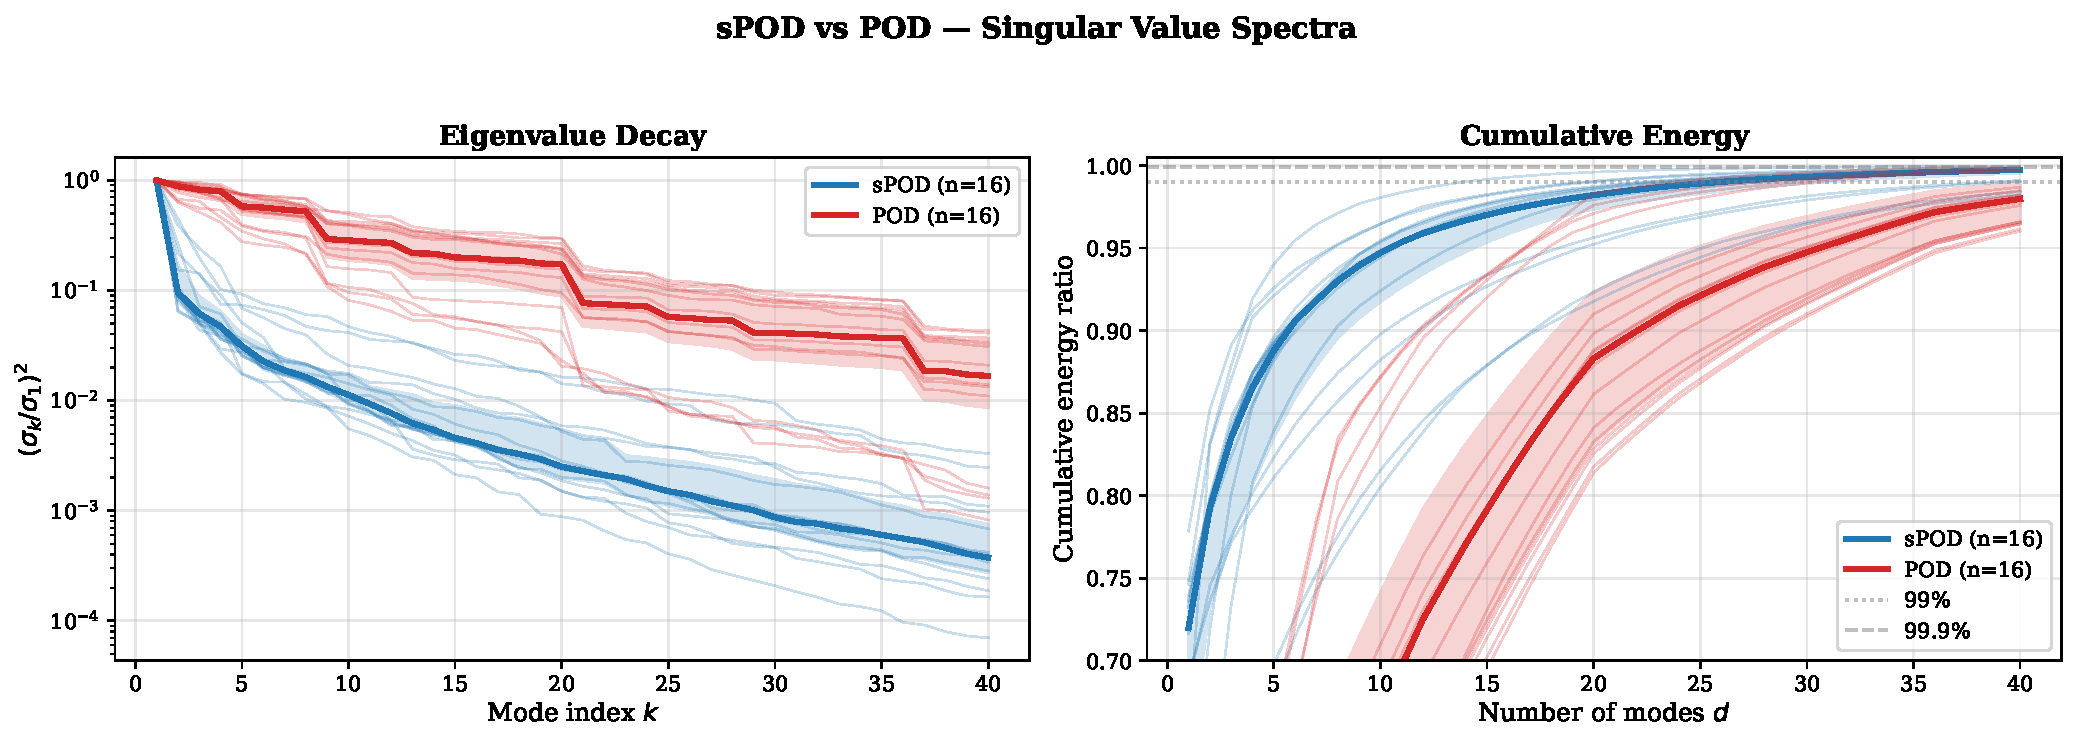
\includegraphics[width=\textwidth]{../Thesis_Figures/thesis_svd_decay.pdf}
\caption{sPOD vs.\ standard POD singular-value spectra aggregated over all
experiments in the catalogue.  Left: normalised eigenvalue decay
$(\sigma_k/\sigma_1)^2$ on a log scale.  Right: cumulative energy ratio.
Thick lines show the cross-experiment mean; shaded bands span individual
runs.  Shift alignment accelerates spectral decay uniformly, supporting a
compact POD truncation at $m=19$ modes.}
\label{fig:spod_vs_pod_decay}
\end{figure}

Because the continuum density evolution
$\partial_t\rho + \nabla\cdot\mathbf{j}=0$ on a periodic domain is
translationally equivariant, the snapshot manifold inherits a continuous
family of near-degenerate directions along group orbits; quotienting
removes these directions while preserving all shape information.  The
choice of reference $\rho_{\mathrm{ref}}$ determines the cross-section;
we use the temporal mean~\eqref{eq:shift_ref}.  This construction is
the discrete, translational-only instance of the more general
\emph{method of slices}~\cite{budanur2015slices,siminos2015periodic}.

\noindent\textbf{Scope and limitations.}
The alignment map is restricted to integer-pixel translations.
It is therefore appropriate for dominant bulk drift, but it does
\emph{not} resolve rotational organisation, multiple simultaneous
transport velocities, deformation of the density envelope, or
topological changes such as merging and splitting of clusters.
This matters especially for variable-speed regimes, where speed
fluctuations produce complex, non-translational density dynamics
(Section~\ref{sec:ch7_shift_dynamics}).

This discrete single-reference alignment is a special case of the
\emph{shifted proper orthogonal decomposition} (sPOD) of
Reiss et~al.~\cite{reiss2018shifted_pod}; the full sPOD machinery
decomposes transport-dominated fields into $K$ co-moving frames via
nuclear-norm minimisation~\cite{krah2024robust_spod,black2020projection}.
More broadly, it connects to diffusion-map separation of symmetry
degrees of freedom~\cite{sonday2011alignment}.

\subsection{Density transform}
\label{subsec:density_transform}

After alignment, a point-wise variance-stabilising transform is applied to
the (positive) density values:
\begin{equation}
  \tilde{\rho} := \sqrt{\rho + \varepsilon},
  \qquad \varepsilon = 10^{-10},
  \label{eq:sqrt_transform}
\end{equation}
The square
root compresses the dynamic range of near-singular density spikes (e.g.\
NDYN05~blackhole) and improves the spectral decay of the snapshot
covariance, so that fewer POD modes are needed to capture a given energy
fraction.  Because the square-root map is nonlinear, it changes both
Euclidean geometry and total transformed mass; exact linear-POD
mass-preservation statements (Section~\ref{sec:mass_preservation})
therefore do not apply prior to inverse transformation.

All subsequent steps---mean computation, centering, SVD, restriction, and
lifting---operate in the \emph{transformed} ($\tilde\rho$) space.  The
inverse transform is applied after lifting:
\begin{equation}
  \hat{\rho} = \bigl[\max(0,\,\hat{\tilde\rho})\bigr]^2 - \varepsilon,
  \label{eq:sqrt_inverse}
\end{equation}
where the clamp to zero guards against small negative values introduced by
POD truncation.

\noindent\textbf{Empirical role in the ROM comparison.}
In the preprocessing ablations, the density transform had little to no
effect on MVAR relative to working directly with raw density snapshots, but
it improved LSTM rollout stability and time-resolved $R^2$ more
consistently across regimes.  Since the thesis compares the mechanistic
WSINDy pipeline against black-box EF-ROM benchmarks, and compares MVAR and
LSTM on a shared latent representation, we retain the same density
transform for both surrogates for like-for-like benchmarking even though
the main benefit is observed on the LSTM side.

%% ===========================================================================
\section{POD via truncated SVD}
\label{sec:pod_svd}

Let $\mathbf{X}\in\mathbb{R}^{T_{\mathrm{tot}}\times d}$ denote the
shift-aligned, $\sqrt{\cdot}$-transformed snapshot matrix.  Compute the
global mean $\boldsymbol{\mu}=\tfrac{1}{T_{\mathrm{tot}}}
\mathbf{X}^\top\mathbf{1}\in\mathbb{R}^d$ and the centred matrix
$\bar{X} := \mathbf{X}^\top - \boldsymbol{\mu}\,\mathbf{1}^\top
\in\mathbb{R}^{d\times T_{\mathrm{tot}}}$.
Compute the thin SVD
$\bar{X} = U\,\Sigma\,V^\top$,
where $U\in\mathbb{R}^{d\times r}$ contains the spatial POD modes,
$\Sigma=\mathrm{diag}(\sigma_1,\dots,\sigma_r)$, and $r=\mathrm{rank}(\bar{X})$.
This matches the construction in Alvarez et~al.~\cite{alvarez2025eqfree};
for a foundational treatment of POD see~\cite{berkooz1993pod}.

\noindent\textbf{Energy spectrum and truncation.}
\label{subsec:energy_truncation}
Define the total energy $E_{\mathrm{tot}}=\sum_{k=1}^r\sigma_k^2$ and
cumulative explained ratio
$\tau(m) := \sum_{k=1}^{m}\sigma_k^2\,/\,E_{\mathrm{tot}}$,
$1\le m\le r$.
In practice we use a \emph{fixed} latent dimension $m=19$
and retain $U_m\in\mathbb{R}^{d\times m}$.
This is a controlled experimental setting for fair cross-regime
comparison; individual truncation optima may differ.  An automatic alternative is the optimal hard threshold of Gavish and Donoho~\cite{gavish2014svht}; the fixed choice adopted here is deliberately conservative.

%% ===========================================================================
\section{Restriction operator \texorpdfstring{$\mathcal{R}$}{R}:
  density \texorpdfstring{$\to$}{to} latent coordinates}
\label{sec:restriction}

In the equation-free setting, restriction is the map
$\mathcal{R}:\mathbb{R}^d\to\mathbb{R}^m$ that takes a (transformed,
centred) snapshot to its latent
coordinates~\cite{alvarez2025eqfree}:
\begin{equation}
  \mathbf{y} = \mathcal{R}(\mathbf{x})
  := U_m^\top\bigl(\mathbf{x}-\boldsymbol{\mu}\bigr)
  \;\in\mathbb{R}^m,
  \label{eq:restriction}
\end{equation}
where $\mathbf{x}=\mathrm{vec}(\tilde\rho)$ is the transformed density.
Thus the latent coordinates parameterise the aligned-and-transformed
snapshot manifold rather than raw physical density fields directly.
In batch form,
$Y = U_m^\top(X - \boldsymbol{\mu}\,\mathbf{1}^\top)
\in\mathbb{R}^{m\times n_t}$.

In the row-stacked implementation, the equivalent
operation is
$\mathbf{Y}_{\mathrm{row}} = (\mathbf{X}-\mathbf{1}\,\boldsymbol{\mu}^\top)\,U_m
\in\mathbb{R}^{T_{\mathrm{tot}}\times m}$,
so that each row of $\mathbf{Y}_{\mathrm{row}}$ is a latent snapshot.

%% ===========================================================================
\section{Lifting operator \texorpdfstring{$\mathcal{L}$}{L}:
  latent \texorpdfstring{$\to$}{to} reconstructed density}
\label{sec:lifting}

Lifting inverts the restriction by projecting back to the POD subspace and
adding the mean:
\begin{equation}
  \hat{\mathbf{x}} = \mathcal{L}(\mathbf{y})
  := U_m\,\mathbf{y} + \boldsymbol{\mu}.
  \label{eq:lifting}
\end{equation}
Since $\boldsymbol{\mu}$ and $U_m$ live in the transformed
($\sqrt{\cdot}$) space, the full reconstruction proceeds in three
conceptually distinct stages: a mathematical lifting step, an inverse
transformation back to density space, and optional admissibility repairs.

\noindent\textbf{Stage~1: Mathematical lifting.}
The latent vector is mapped back to the POD subspace:
$\hat{\mathbf{x}} = U_m\,\mathbf{y}+\boldsymbol{\mu}$
(in $\sqrt{\rho}$ space).

\noindent\textbf{Stage~2: Inverse transform to density space.}
The square-root map is inverted to recover physical density:
$\hat\rho = [\max(0,\hat{\mathbf{x}})]^2 - \varepsilon$
(Eq.~\ref{eq:sqrt_inverse}), where the clamp guards against small
negatives introduced by POD truncation.

\noindent\textbf{Stage~3: Optional admissibility postprocessing.}
Two optional corrections restore basic physical admissibility---chiefly
nonnegativity and total mass---that may be lost under the nonlinear
transform and forecast error:
\begin{itemize}[nosep]
  \item \emph{Nonnegativity clamp}: $\hat\rho^{+} \leftarrow \max(\hat\rho,0)$.
  \item \emph{Mass correction}: either global rescaling
        $\mathcal{S}_{M_0}$ (Eq.~\ref{eq:mass_postprocess_scale}) or
        simplex projection $\Pi_{\Delta^{d-1}_{M_0}}$ (Eq.~\ref{eq:mass_postprocess_simplex}),
        where $M_0 := \sum_{j=1}^{d}\rho_j(t_{n_0})$ is the true mass
        at forecast start.
\end{itemize}
Finally, the spatial shift is undone:
$\hat\rho_{2\mathrm{D}}
\leftarrow \mathrm{roll}(\hat\rho_{2\mathrm{D}},\;
-\Delta y_k,-\Delta x_k)$.

The two mass-correction operators are defined as
{\setlength{\abovedisplayskip}{5pt}
\setlength{\belowdisplayskip}{5pt}
\begin{align}
  \Pi_{\Delta^{d-1}_{M_0}}(\hat\rho)
  &:= \arg\min_{\rho\in\Delta^{d-1}_{M_0}}
  \|\rho-\hat\rho\|_2^2,
  \label{eq:mass_postprocess_simplex}\\
  \mathcal{S}_{M_0}(\hat\rho)
  &:=
  \begin{cases}
    \hat\rho\,\dfrac{M_0}{\sum_{j=1}^{d}\hat\rho_j},
    & \text{if }\sum_{j=1}^{d}\hat\rho_j > 0,\\[6pt]
    \hat\rho,
    & \text{otherwise,}
  \end{cases}
  \label{eq:mass_postprocess_scale}
\end{align}
}
where $\Delta^{d-1}_{M_0}:=\{\rho\in\mathbb{R}^d:\rho_j\ge0,\;\sum_j\rho_j=M_0\}$.
In preliminary ablations, both operators had negligible effect on MVAR
forecast quality but improved LSTM rollout stability.
All reported results use mass rescaling paired with
the nonnegativity clamp, which gave slightly higher $R^2$ in the final
ablation round; results with simplex projection were comparable.

%% ===========================================================================
\enlargethispage{2\baselineskip}
\section{Mass preservation under linear POD}
\label{sec:mass_preservation}

When no density transform is applied (i.e.\ the pipeline is purely linear),
POD lifting preserves total mass exactly.
This is a standard property of mean-centred orthogonal projections; a proof
for the normalised-density case in the crowd-dynamics setting appears in
Alvarez et~al.~\cite[Proposition~1]{alvarez2025eqfree}.
We give a self-contained argument below, generalised to arbitrary
constant mass~$M_0$ and written in the notation of our pipeline
(Sections~\ref{sec:pod_svd}--\ref{sec:lifting}).

\begin{proposition}[Mass preservation under constant-mass snapshots]
\label{prop:mass_preservation}
Let $X=[x_1,\dots,x_{n_t}]\in\mathbb{R}^{d\times n_t}$ with
$\mathbf{1}^\top x_k = M_0$ for all~$k$.
Let $\bar{X}=XH$, $\bar{X}=U\Sigma V^\top$, and define the reconstruction
$\tilde{X}:=U_m U_m^\top\bar{X}+\boldsymbol{\mu}\mathbf{1}^\top$.
Then $\mathbf{1}^\top\tilde{x}_k=M_0$ for all~$k$.
\end{proposition}

\begin{proof}
Write the reconstruction column-wise:
$\tilde{x}_k = U_m U_m^\top \bar{x}_k + \boldsymbol{\mu}$,
where $\boldsymbol{\mu} = \frac{1}{n_t}X\mathbf{1}$ is the snapshot mean.
Summing $\boldsymbol{\mu}$ gives
$\mathbf{1}^\top\boldsymbol{\mu}
 = \frac{1}{n_t}\mathbf{1}^\top X\mathbf{1}
 = \frac{1}{n_t}\cdot n_t M_0 = M_0$.
It therefore suffices to show that the projection term contributes zero mass.
Because every column of~$\bar{X}$ sums to zero
($\mathbf{1}^\top\bar{x}_k = \mathbf{1}^\top x_k - M_0 = 0$),
the constant vector $\mathbf{1}$ lies in the left null-space
of~$\bar{X}$.
Every column of~$U_m$ is a left singular vector of~$\bar{X}$ and thus
belongs to its column space, so
$\mathbf{1}^\top U_m = \mathbf{0}^\top$.
Hence
$\mathbf{1}^\top(U_m U_m^\top\bar{x}_k) = \mathbf{0}^\top\bar{x}_k = 0$
and $\mathbf{1}^\top\tilde{x}_k = 0 + M_0$.
\end{proof}

\begin{remark}[Effect of the density transform]
Proposition~\ref{prop:mass_preservation} applies to the purely
linear pipeline only and does not extend to the full square-root pipeline.
The $\sqrt{\cdot}$ transform is nonlinear: even if
$\sum_j\rho_j=M_0$ for all frames, the transformed snapshots
$\tilde\rho_j=\sqrt{\rho_j+\varepsilon}$ do \emph{not} share a common mass.
Proposition~\ref{prop:mass_preservation} therefore does not apply in the
transformed space, and an optional mass correction operator
(rescaling or simplex projection) is used to restore physical
mass after inverse transformation.  Proposition~\ref{prop:mass_preservation}
nevertheless motivates the expectation that mass drift should be small even
in the nonlinear pipeline, and explains why only mild post-processing
corrections are needed in practice.
\end{remark}

%% ===========================================================================
Algorithm~\ref{alg:pod_pipeline}
(Appendix~\ref{app:detailed_algorithms}) gives the complete pseudocode
for the global POD restriction--lifting pipeline.

\noindent
Algorithm~\ref{alg:pod_pipeline} describes the pipeline used in
all experiments; Proposition~\ref{prop:mass_preservation}, by contrast,
describes an idealised linear special case that clarifies the source of
exact mass preservation.

\noindent
\textbf{What the ROM pipeline preserves and what it discards.}
The restriction--lifting pipeline deliberately quotients out coherent
translational drift (via shift alignment) and compresses the aligned density
movie to $m=19$ latent coordinates (via truncated SVD), retaining the
dominant spatial modes while discarding fine-scale structure below the
truncation threshold.  The resulting latent space is therefore a controlled
compression of the aligned density manifold, not a physically closed state
description: it contains information only about mass-density shape modes,
not about the auxiliary fields (polarisation flux, Morse potential) that
WSINDy uses for mechanism identification.  Whether the latent dynamics are
effectively linear under this representation, or whether substantial
nonlinear memory remains, is the question addressed by the MVAR/LSTM
comparison in Chapter~\ref{ch:latent_rom}.
